\documentclass[tikz,border=4pt]{standalone}
\usepackage[T1]{fontenc}
\usepackage{lmodern,amsmath,amssymb}
\usetikzlibrary{arrows.meta,calc}
\begin{document}
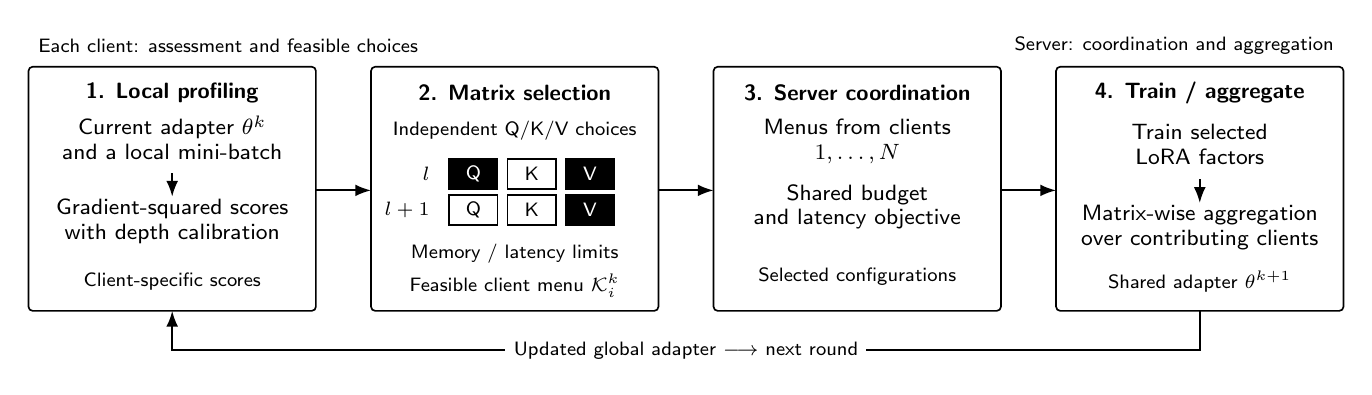
\begin{tikzpicture}[x=1cm,y=1cm,font=\sffamily\fontsize{8}{9}\selectfont,
  box/.style={draw=black,line width=.6pt,rounded corners=1.5pt,fill=white},
  flow/.style={-{Latex[length=2mm]},line width=.7pt},
  tinybox/.style={draw=black,line width=.5pt,minimum width=.62cm,minimum height=.38cm,inner sep=1pt,font=\sffamily\fontsize{7.4}{8.3}\selectfont}]
\foreach \x in {0,4.35,8.70,13.05}{\draw[box] (\x,.65) rectangle ++(3.65,3.1);}
\node[font=\sffamily\fontsize{8}{9}\selectfont\bfseries] at (1.825,3.42) {1. Local profiling};
\node[font=\sffamily\fontsize{8}{9}\selectfont\bfseries] at (6.175,3.42) {2. Matrix selection};
\node[font=\sffamily\fontsize{8}{9}\selectfont\bfseries] at (10.525,3.42) {3. Server coordination};
\node[font=\sffamily\fontsize{8}{9}\selectfont\bfseries] at (14.875,3.42) {4. Train / aggregate};
\node[align=center] at (1.825,2.85) {Current adapter $\theta^k$\\and a local mini-batch};
\draw[flow] (1.825,2.40)--(1.825,2.10);
\node[align=center] at (1.825,1.78) {Gradient-squared scores\\with depth calibration};
\node[font=\sffamily\fontsize{7.4}{8.3}\selectfont] at (1.825,1.02) {Client-specific scores};
\node[font=\sffamily\fontsize{7.4}{8.3}\selectfont] at (6.175,2.94) {Independent Q/K/V choices};
\node[font=\sffamily\fontsize{7.4}{8.3}\selectfont,anchor=east] at (5.22,2.39) {$l$};
\node[font=\sffamily\fontsize{7.4}{8.3}\selectfont,anchor=east] at (5.22,1.93) {$l+1$};
\node[tinybox,fill=black,text=white] at (5.65,2.39) {Q};
\node[tinybox] at (6.39,2.39) {K};
\node[tinybox,fill=black,text=white] at (7.13,2.39) {V};
\node[tinybox] at (5.65,1.93) {Q};
\node[tinybox] at (6.39,1.93) {K};
\node[tinybox,fill=black,text=white] at (7.13,1.93) {V};
\node[font=\sffamily\fontsize{7.4}{8.3}\selectfont] at (6.175,1.38) {Memory / latency limits};
\node[font=\sffamily\fontsize{7.4}{8.3}\selectfont] at (6.175,.97) {Feasible client menu $\mathcal K_i^k$};
\node[align=center] at (10.525,2.80) {Menus from clients\\$1,\ldots,N$};
\node[align=center] at (10.525,1.97) {Shared budget\\and latency objective};
\node[font=\sffamily\fontsize{7.4}{8.3}\selectfont] at (10.525,1.08) {Selected configurations};
\node[align=center] at (14.875,2.76) {Train selected\\LoRA factors};
\draw[flow] (14.875,2.32)--(14.875,2.02);
\node[align=center] at (14.875,1.71) {Matrix-wise aggregation\\over contributing clients};
\node[font=\sffamily\fontsize{7.4}{8.3}\selectfont] at (14.875,1.02) {Shared adapter $\theta^{k+1}$};
\foreach \a/\b in {3.65/4.35,8/8.70,12.35/13.05}{\draw[flow] (\a,2.18)--(\b,2.18);}
\draw[flow] (14.875,.65)--(14.875,.15)--(1.825,.15)--(1.825,.65);
\node[fill=white,inner sep=3pt,font=\sffamily\fontsize{7.4}{8.3}\selectfont] at (8.35,.15) {Updated global adapter $\longrightarrow$ next round};
\node[font=\sffamily\fontsize{7.4}{8.3}\selectfont,anchor=west] at (0,4.02) {Each client: assessment and feasible choices};
\node[font=\sffamily\fontsize{7.4}{8.3}\selectfont,anchor=east] at (16.70,4.02) {Server: coordination and aggregation};
\end{tikzpicture}
\end{document}
